\chapter{Testing and evaluation}
\label{cha:testing}

The initial plan was to have a total of 10 participants to take part in a 2-hour testing process. However, some people dropped out while other people expressed interest, so the final number of participants was 13. All the participants were university students. The testing took place in week 4 of second semester, more precisely 17th to 20th of February.

At the moment of user testing, the game was finished with the exception of the car model and colour choice.

In this chapter, we are going to discuss the results of the user testing. The used questionnaire can be found in appendix \ref{appendix:userStudy}. 

For the purposes of testing the projects, the participants were firstly asked to play the game in keyboard mode. Following this, they were asked to fill in a NASA TLX (Task Load Index) test so that we would have a measurement of how demanding this task was for the user. Next, the Emotiv EPOC headset was fit on the participant's head and the training process would begin. After feeling confident enough for the first action (push), the user could see it working in the actual game play. We insisted on properly training 2 actions: push - for acceleration - and left - for a left turn. The reason why left was necessary is because the track does a left turn on a slightly elevated terrain. Less than 5 users have probably had enough time to train the other 2 states (pull and right) as well. Again, after the 2 hours were almost up, the participant was asked to take another NASA TLX test, this time taking into account how demanding the process was for Cognitiv game play. Finally, the participant was asked to fill in the user study questionnaire in appendix \ref{appendix:userStudy}. 

The following sections will describe the results of the user testing. In section \ref{section:implemented}, we will highlight what was changed in CogniDriver following the participants' answer, in the period of 2 weeks left before the project demonstrations period begun.

\section{Observations}

Some of the participants displayed better skill in training the headset if the testing was done in the morning. This is compared to evenings, when some of the partipants complained about being tired and not being able to concentrate properly.

The testing was done using a cube as the training object. In my opinion, this would have made training consistent with people used to the Emotiv EPOC Control Panel or other applications which require Cognitiv training. 

It may be difficult to switch to a different mental state when training a new action. As a result, new training data for an action, might override data for a previous action. This happened to me a few times and it did happen with some of the participants as well.

When training or playing the game, if the car is being moved, the enthusiasm generated by that may make the player lose concentration.

\section{NASA TLX results}
The test was taken using the \cite{nasatlx} online version developed by Keith Vertanen. It produces the analysis of the input data for each person at the end of the test. 

For keyboard mode, the overall mean difficulty was 51.611\% with a standard deviation of 17.494\%.

For Cognitiv mode, the overall mean difficulty was 90.571\% with a standard deviation of 13.964\%.

This tells us the participants have found the game much easier to play in keyboard mode compared to Cognitiv mode which was very demanding.

\section{Analysis of user questionnaire answers}
The user questionnaire aimed to measure things such as the comfort of wearing the headset and how demanding the training and playing were, especially in Cognitiv mode.

The mean of the comfort of wearing the headset was 5.692 out of 10 with an approximately equal spread of scores. Most of the participants have started feeling the discomfort after 20-40 minutes of wearing the headset. 

For the questions regarding the demand of the process, the participants' scores were quite unanimous. The training demand obtained a score of 4.23/10, the play demand obtained a score of 3.153/10 and the ease demand obtained 2.153/10. The similarity between the keyboard play and Cognitiv play was of 2.307/10 suggesting the two modes are not similar.

\section{Good points about the game}
The first point to make was that users found it easy to focus on the task because driving is a real life skill and it is easy to understand. Many times, participants made correlations between the driving game and the real life skill.

Raining when frustrated was considered a great feature by most.

The graphics were generally appreciated and feedback was received on the track as being sensible. 

Some players enjoyed the funny game physics because there were opportunities for cheating. However, these opportunities have been reduced now and we have tried improving the physics so that not as much skidding would occur.

The training interface was considered clear and understandable.

\section{Bad points about the game}
It was hard to tell which way is the right direction of driving if the car skid and the player got disorientated.

The car accelerated too fast and some of the game physics were peculiar. 

Some considered it would have been useful to see the brainwaves for each channel since this might have provided more feedback on how the training was going and how to concentrate on completing the task.

The training process requires concentration and it can take a long time. Some people were disturbed by the amount of clicking going on in order to start training, accept or reject it and then start again. It also got the participant distracted and it was breaking the concentration level. Sometimes, I would do the clicking for the participant so I could catch the events when the object was really being moved. Complaints were received regarding the training as being too stressful, frustrating and not rewarding. The amount of clicking, although disliked by many, is not something which could be changed since the training process can vary in duration. It was suggested that an approach to this might be to automatically accept a training if it meets some set guidelines but then the participant is quite out of control of the process. In addition, it might make the movement more difficult to control.

Some invisible colliders\footnote{An invisible object that is used either as a barrier to stop another object from going through it or which is used as a trigger to detect whether another object has reached that point} from around the mountains were slightly touching the road side. This has now been fixed.

The driver seat view was not always enjoyable, especially when the sensor contact quality was not perfect and the blink would be mistaken for a left wink which would then cause the camera view to change.

\section{What should be improved and what has been implemented?}
\label{section:implemented}
It has been suggested by more than a half of the participants that training would be easier if it was done with a car object rather than a cube as this made them more properly visualise the action. It also made it easier to activate an action while playing the game. This has been implemented.

Checkpoints were another suggestion so that players could be stopped from cheating and taking a short route to the finish line. This has been implemented with the help of invisible colliders which were being triggered when the car would pass through them. A total of 17 checkpoints have been inserted. At the finish line, if the number of checkpoints the player has been through is different than 17, the message in figure \ref{fig:ohno} will appear, giving the option to restart the game.

\begin{figure}
  \centering
  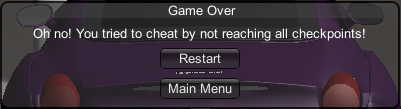
\includegraphics[width=300px]{ohno.png}
  \caption{A print screen of the message which will occur in case the player tries to follow a shortcut to the finish line}
    \label{fig:ohno}        
\end{figure}

The current action used to be displayed as text, but the suggestion was to have a system of arrows being highlighted for each type of movement. This has been implemented.

One suggestion was to add some coins to the road that the player could collect. This has been implemented and it solves the issue of the users not knowing which is the right direction of going. It also obliges the player to stick more to the centre of the road and it provided an extra way of deciding the highscores, besides the elapsed time.  

There used to be a quite annoying reverse sound which was suggested to be removed by the majority of participants. It was seen as distracting when the player was trying to concentrate on the action. The motor sound though, did not seem as stressful.

There used to be no way of restarting the race from the keyboard. This is now done when the player is pressing the 'R' key. Also, using 'T' will make the car respawn at the last checkpoint it has been through just in case the player gets lost around the environment. It is not something that should happen too often, but it might occur.

The things which have not been implemented had to do with not having access to the raw EEG data or them simply not being feasible or important.

From a talk after the testing session was complete, it was suggested it would be good to give the car different speeds on grass and road. This has been implemented. The car accelerates about 2 times slower when it gets on the grass area.